\documentclass[10pt]{beamer}
\usetheme[progressbar=frametitle]{metropolis}

\usepackage [autostyle, english = american]{csquotes}
\DeclareFontShape{OT1}{cmss}{b}{n}{<->ssub * cmss/bx/n}{} 
\usepackage{amsmath}
\usepackage{amssymb}
\usepackage{bm} 
\usepackage{multicol}

\MakeOuterQuote{"}
\newcommand{\imp}[1]{\textbf{\color{cyan}#1}}

%---------------------------------------------------
% Title 

\title{Refining Character Relationships in a Textual Narrative using Embeddings of Interactions}
\date{}
\author{Guillaume Guex}
\institute{University of Lausanne}

\begin{document}
	
	%------------------------------------------------------------------
	
	\maketitle
	
	%------------------------------------------------------------------
	
	\begin{frame}{Table of contents}
		\setbeamertemplate{section in toc}[sections numbered]
		\tableofcontents%[hideallsubsections]
	\end{frame}

	%------------------------------------------------------------------
	
	\section[Introduction]{Introduction}
	
	%------------------------------------------------------------------
	
	\begin{frame}{The construction of a character network}
		The construction of a character network takes generally 3 steps \cite{labatut_extraction_2019}:
		\begin{itemize}
			\item Identification of \imp{characters} 
			\item Detection of \imp{interactions}
			\item Construction of the \imp{graph}
		\end{itemize}
	\end{frame}

	%------------------------------------------------------------------
	
	\begin{frame}{The construction of a character network}
		When dealing with \imp{textual narrative}, a frequently used method is to count \imp{character co-occurrences} in \imp{textual units} (e.g., \cite{elsner_character-based_2012, rochat_analyse_2014}). \\
		\vspace{-0.4cm}
		\begin{columns}
			\begin{column}{0.5\textwidth}
				\begin{figure}
					\centering
					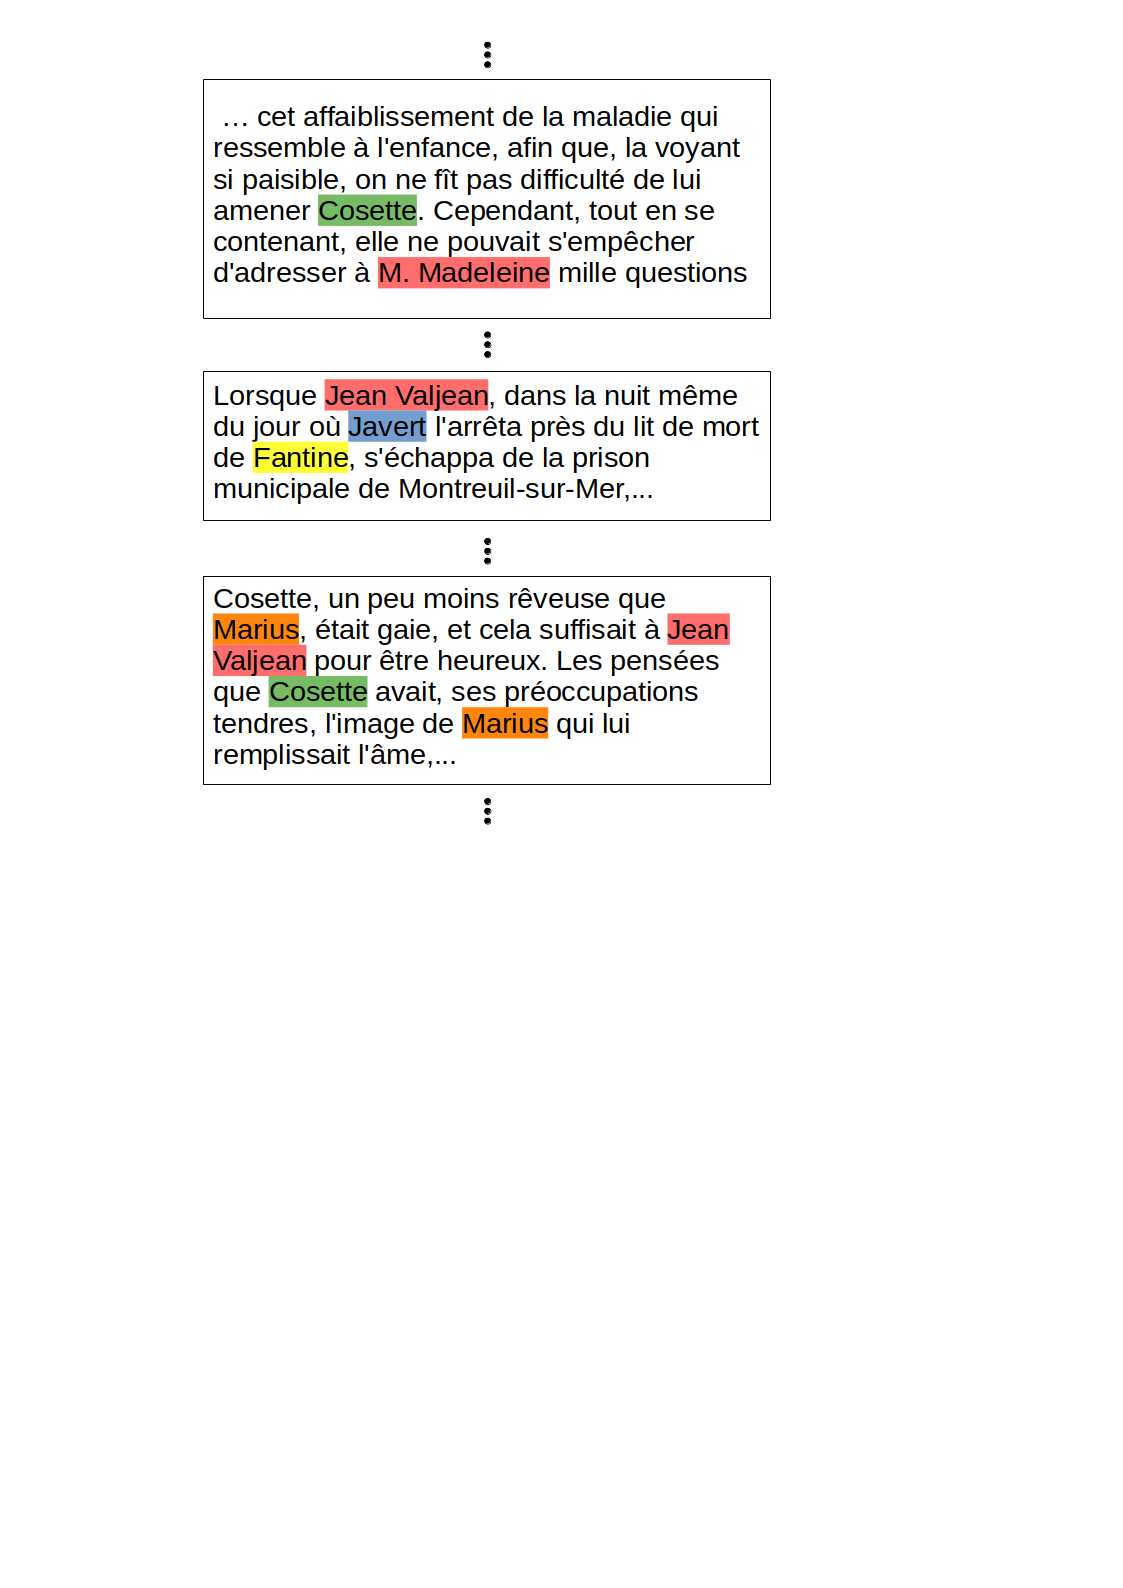
\includegraphics[width=1.4\textwidth]{img/textual_units.png}
				\end{figure}
			\end{column}
			\begin{column}{0.5\textwidth}
				\vspace{-4cm}
				\begin{table}
					\centering
					\scriptsize
					\begin{tabular}{|c|c|c|} 
						\hline
						Character 1 & Character 2 & Co-occurrences \\ 
						\hline
						Cosette & Marius & 1 \\
						Cosette & Valjean & 2 \\ 
						Fantine & Javert & 1 \\
						Fantine & Valjean & 1 \\
						Javert & Valjean & 1 \\
						Marius & Valjean & 1 \\
						\hline
					\end{tabular}
				\end{table}
				\begin{figure}
					\centering
					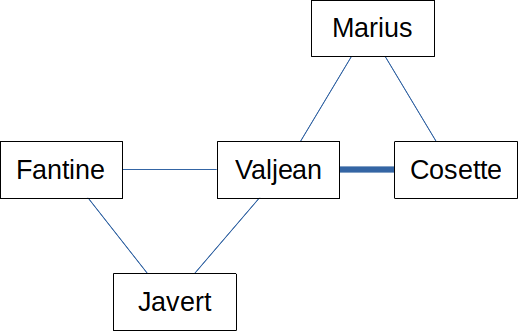
\includegraphics[width=0.8\textwidth]{img/mini_graph.png}
				\end{figure}
			\end{column}
		\end{columns}
	\end{frame}
	
	%------------------------------------------------------------------
	
	\begin{frame}{Dataset}
		In this context, the \imp{dataset} used to construct the character network has the following form
		\begin{figure}
			\centering
			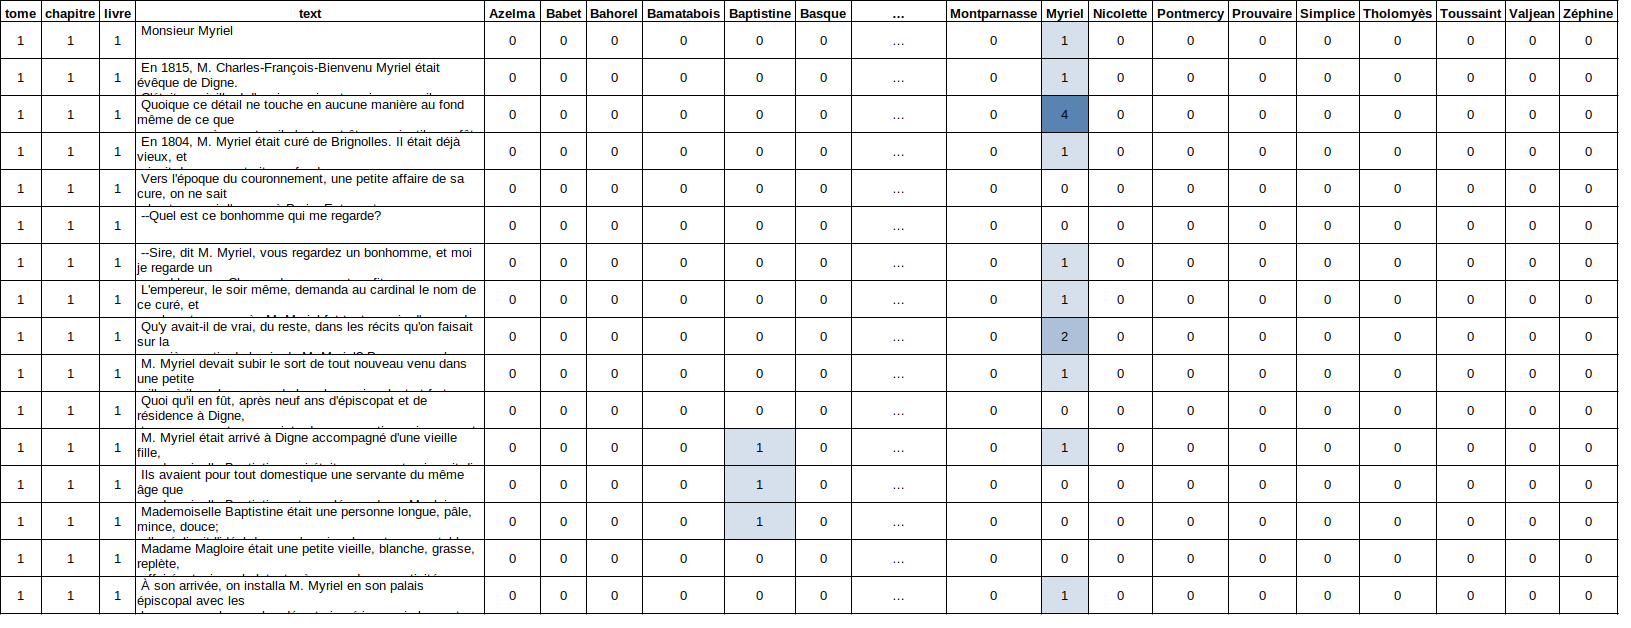
\includegraphics[width=\textwidth]{img/data_table.png}
		\end{figure}
		However, apart from a few exceptions \cite{nalisnick_character--character_2013, trovati_towards_2014, min_modeling_2019}, the content of the \imp{text column} is not used. \imp{Edges in the resulting graph aggregate blindly various kind of interactions}.
	\end{frame}
	
	
	%------------------------------------------------------------------
	
	\begin{frame}{Approaches}
		In this presentation, we propose to \imp{refine character relationships} by using the \imp{textual data}. Quantities of approaches can be undertaken, but we focus on:
		\begin{itemize}
			\item \imp{Bag-of-paths} approaches, a corpus is represented by an \imp{unit-term matrix}. \\
			\vspace{0.3cm}
			\begin{figure}
				\centering
				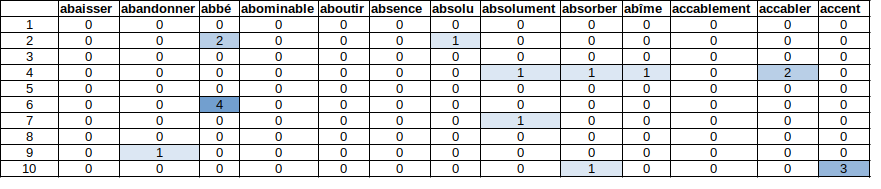
\includegraphics[width=0.8\textwidth]{img/unit_term.png}
			\end{figure}
			\item \imp{Embeddings of textual units}. The unit-term matrix is used to construct \imp{vectors} representing units. 
			\item \imp{Embeddings of character relationships}, which derives from the embedding of textual unit.
		\end{itemize}
	\end{frame}
	
	
	%------------------------------------------------------------------
	
	\begin{frame}{Approaches}
		More specifically, three approaches are made:
		\begin{itemize}
			\item \imp{Correspondence Analysis (CA)}.
			\item \imp{Pre-trained Word Embeddings (WE)}.
			\item "Topic" vectors from \imp{Non-negative Matrix Factorization (NMF)}.
		\end{itemize}
	\end{frame}
	
	
	%------------------------------------------------------------------
	
	
	\section[Correspondence Analysis (CA)]{Correspondence Analysis (CA)}
	
	%------------------------------------------------------------------
	
	\begin{frame}{Principles}
		Correspondence Analysis is the natural tool for analyzing textual resources if data are organized in a $(n \times p)$ \imp{document-term matrix} \cite{lebart_analyse_2019} (here, documents are our textual units). It gives:
		\begin{itemize}
			\item $\min(n, p) - 1$ \imp{factorial axes}, by decreasing order of importance, which can be interpreted as latent variables.
			\item \imp{Coordinates of each document} along these factors, where proximity can be interpreted as similar profile in term of words.
			\item \imp{Coordinates of each word} along the same factors, where proximity can be interpreted as similar profile in term of documents.
			\item \imp{Affinities between a document and a term}, which is computed by the \imp{scalar product} between their vectors.
		\end{itemize}
	\end{frame}
	
	%------------------------------------------------------------------
	
	\begin{frame}{Principles}
		If we plot units and words on the first two axes, we get the usual \imp{biplot}:
		\begin{figure}
			\centering
			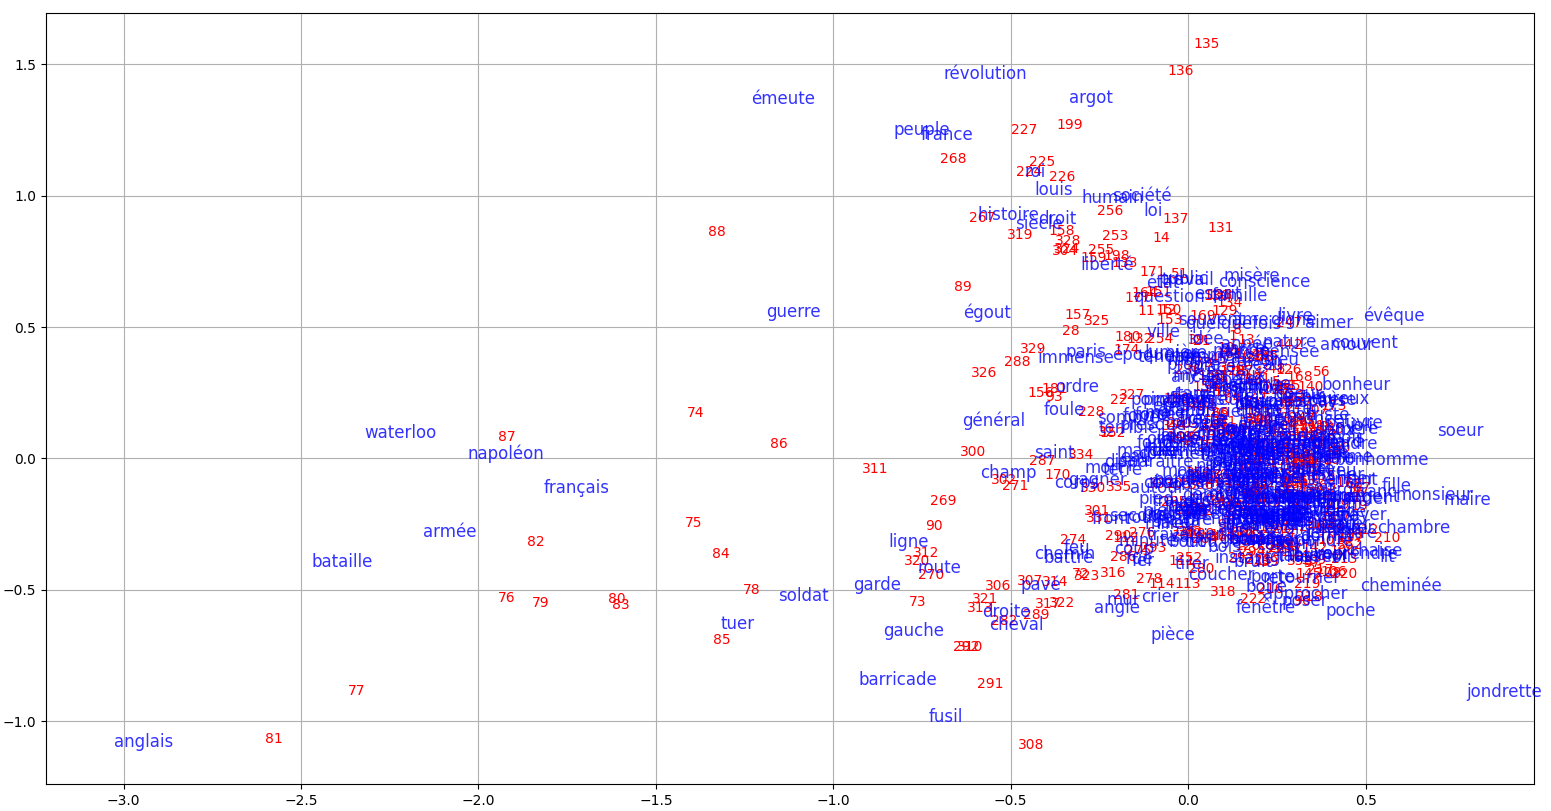
\includegraphics[width=\textwidth]{img/biplot.png}
		\end{figure}
	\end{frame}
	
	%------------------------------------------------------------------
	
	\begin{frame}{Relationship embeddings}
		If we plot units and words on the first two axes, we get the usual \imp{biplot}:
		\begin{figure}
			\centering
			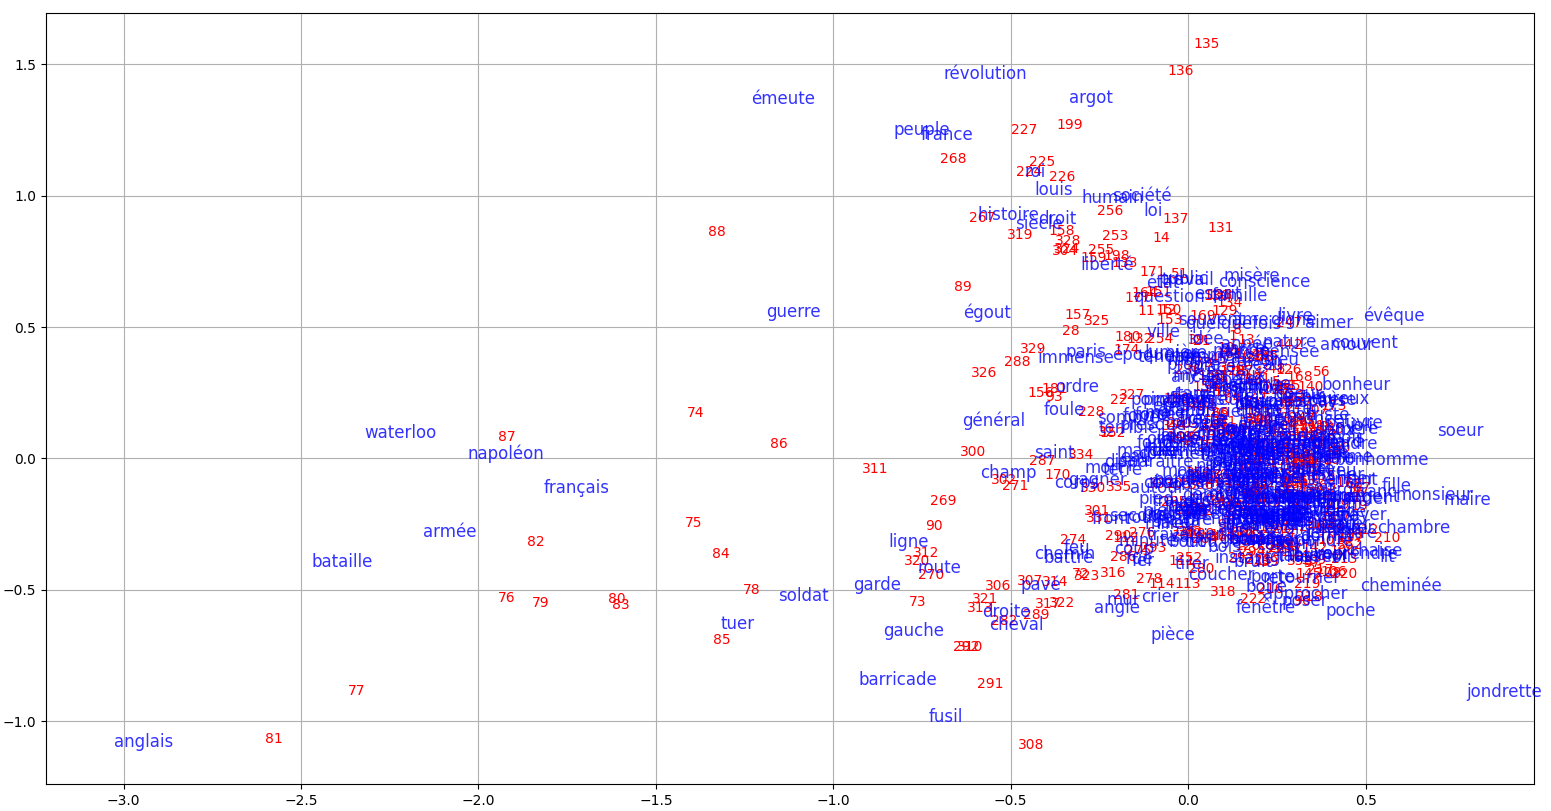
\includegraphics[width=\textwidth]{img/biplot.png}
		\end{figure}
	\end{frame}
	
	%------------------------------------------------------------------
	
	\appendix
	
	\begin{frame}[shrink=40, fragile]{References}
		\begin{multicols}{2}
			\bibliographystyle{apalike}
			\bibliography{charnet}
		\end{multicols}
	\end{frame}
	
\end{document}
